\documentclass[12pt]{article}


\usepackage{graphicx}
\graphicspath{ {./Figures/} }
\usepackage{amsmath}
\usepackage{amsfonts}
\usepackage{hyperref}

\title{Variational Inference Framework for Compartmental Disease Transmission Models}

\author{GitHub: \url{https://github.com/epidemic-research-team/}}

\begin{document}
\maketitle

\section{Introduction}

\section{Model Goals Overview}

The goal of this research is to utilise Variational Inference methods in order to increase the computational efficiency of the \cite{Gareth:2013} paper. 

\begin{itemize}
\item Approximate the posterior 
\item Apply VI methods on non-linear ODE system
\item Evaluate the results
\end{itemize}

\section{Literature Review}

\begin{itemize}
\item Hensman, 2016 - Variational Bayesian non-Parametric Inference for Infectious Disease Models
\item Blei, 2016 - Variational Inference: A Review for Statisticians
\end{itemize}


\section{Method}

\subsection{ODE system model}

The compartmental transmission model from \cite{Gareth:2013} has a form as shown in Figure \ref{fig:model} \cite[p.5]{Gareth:2013}. 

\begin{figure}[h!]
\centering
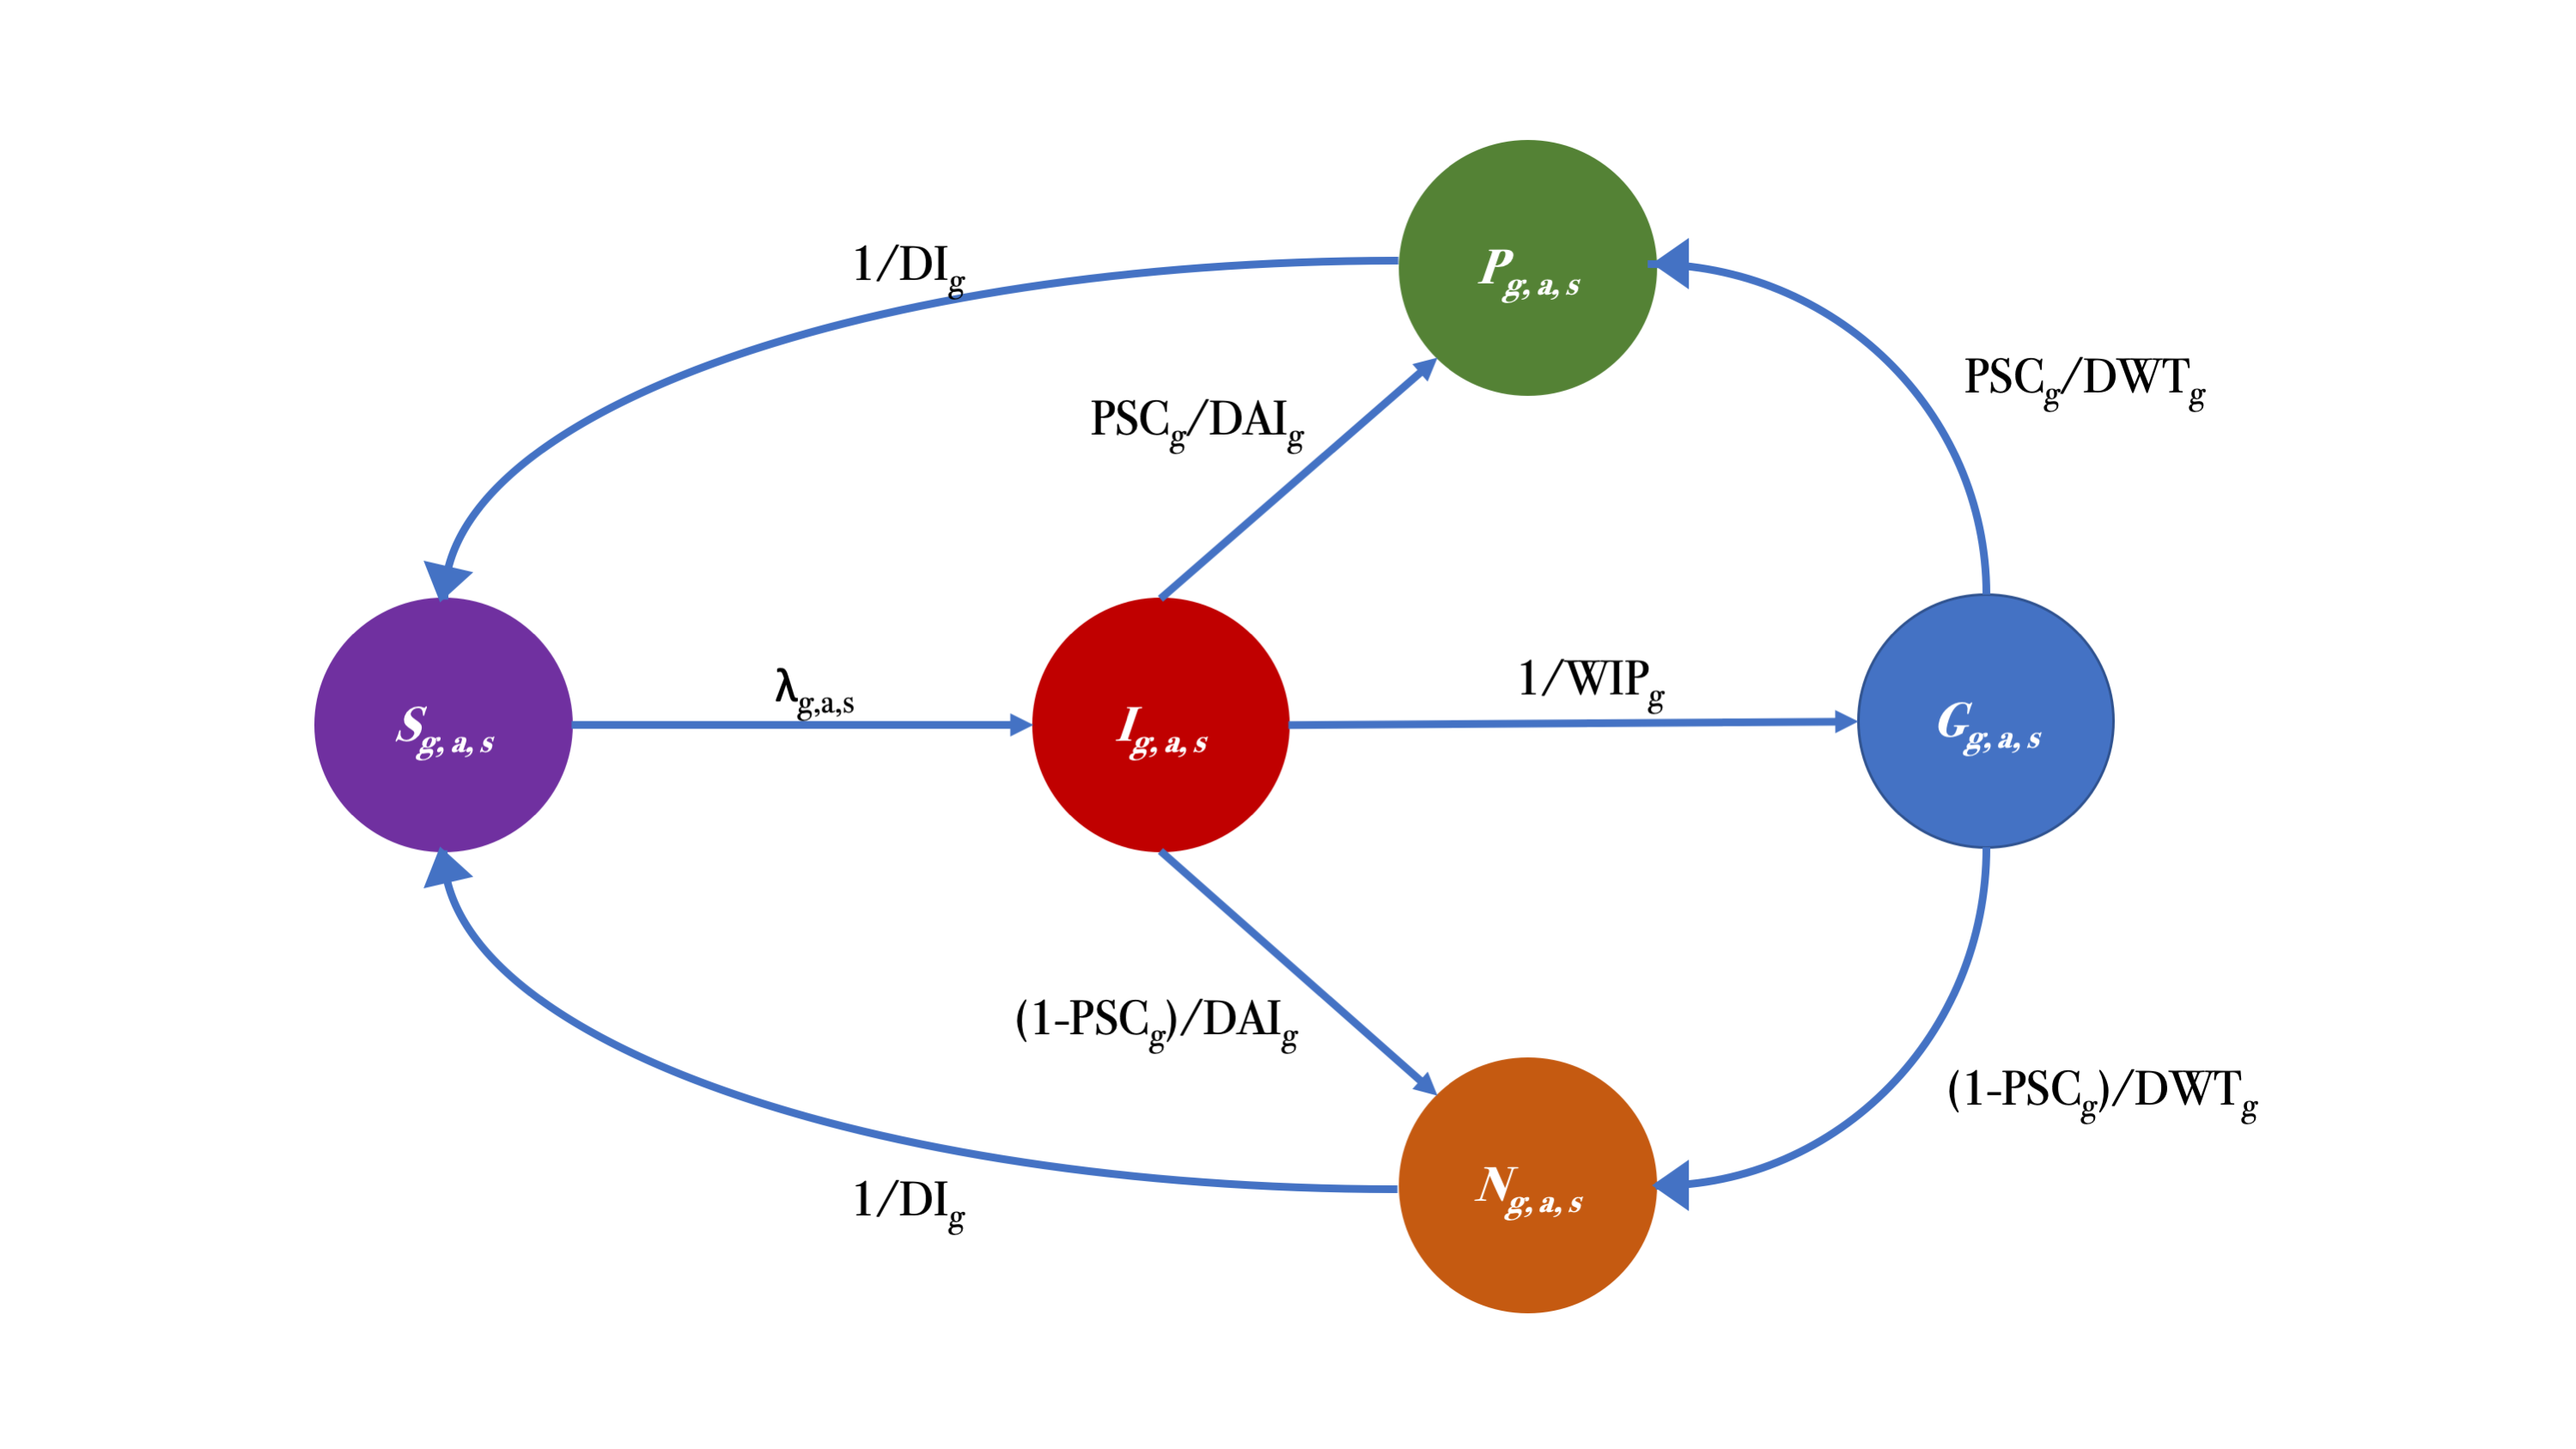
\includegraphics[width=1\textwidth]{COVIDb}
\caption{A compartmental Covid-19 transmission model.}
\label{fig:model}
\end{figure}

We modify the original model by removing the indices $g$ and $s$ that indicate gender and level of social activity and retaining only the age related groups $a$, 19 age-groups in total. The system of ODEs is formulated as follows

\begin{align}
\label{eq:ODE}
\dot{S}_{a} & =  -\lambda_{a}(t)S_{a} + (P_{a} + N_{a})/DI + \frac{1}{r}S_{a-1} - \frac{1}{r}S_{a} + \\ \nonumber
& \quad \frac{1}{R}(S_{19} + I_{19} + G_{19} + P_{19} + N_{19}) \times \\ \nonumber
& \quad \delta_1(a)(\pi_1\delta_1(s) + \pi_2\delta_2(s) + \pi_3\delta_3(s) + \pi_4\delta_4(s)) \\ 
\dot{I}_{a}  & =  \lambda_{a}(t)S_{a} - (1/WIP + 1/DAI)I_{a} + \frac{1}{r}I_{a-1}-\frac{1}{r}I_{a} \\ 
\dot{G}_{a}  & =  I_{a}/WIP - G_{a}/DWT + \frac{1}{r}G_{a-1} - \frac{1}{r}G_{a} \\ 
\dot{P}_{a}  & =  PSC(I_{a}/DAI + G_{a}/DWT) - P_{a}/DI + \frac{1}{r}P_{a-1} - \frac{1}{r}P_{a} \\
\dot{N}_{a}  & =  (1-PSC)(I_{a}/DAI + G_{a}/DWT) - N_{a}/DI + \frac{1}{r}N_{a-1}-\frac{1}{r}N_{a} \\ \nonumber
\end{align}

From the Figure \ref{fig:model}, there are 5 non-overlapping compartments: $S$ is for individuals who are at risk of Covid-19 infection, $I$ is for infected individuals, $G$ is for infected who developed serious symptoms and required ICU admission, $P$ is for those who have recovered, and are seropositive and immune, $N$ is for individuals who are recovered, immune but seronegative. Movements between compartments are occurring at per capita rates specified by the following parameters: \textbf{PSC} is the probability of becoming seropositive, \textbf{WIP} is the Covid-19 incubation period, \textbf{DAI} is the duration of asymptomatic (i.e. without Covid-19) infection symptoms, \textbf{DWT} is the duration of treatment for Covid-19, and \textbf{DI} is the duration of immunity. Subscripts denote stratification of parameters: for example, $dot{I}_{a}$ means that in our model this variable is age-dependent. Finally, $\lambda$ is the \textbf{force of infection} and is defined as

\begin{equation}
\lambda_{a}(t)=\sum_{a^{'}} \bigg\{ M(t) \frac{I_{a'}(t)}{S_{a'}(t) + I_{a'}(t) + G_{a'}(t) + N_{a'}(t) + P_{a'}(t)} \bigg\}
\end{equation}

with $M$ a time-varying social mixing matrix, constructed by combining social information from the BBC Pandemic project\footnote{For more information about the data and the construction of the social mixing matrix the reader should refer to the Social Mixing Matrix Literature Review and an Intuitive Approach for the $\mathcal{R}_{0}$} and from the Google mobility reports.

\subsection{Model Inputs}

Let $X$ be a time dependent vector that includes the 5 states of the compartmental model, with $X_{a}(t)=[S_{a}(t), I_{a}(t), G_{a}(t), P_{a}(t), N_{a}(t)]$ and $t \in \{1,2,\dots,T \}$. Also, assume that the observations of the model for time $t$ are $D_{a}(t)$ as the number of infected.

\subsection{Priors}

Next step, we replicate  work on a Bayesian modelling framework that will involve the treatment the parameters of the non-linear system of ODE equations describing the epidemic as unknown random variables. In total, Gareth et al. model \cite{Gareth:2013} has 7 parameters with their relevant priors (Table \ref{table:priors})

\begin{table}[h!]
\centering
 \begin{tabular}{||l c r||} 
 \hline
 Parameter & Interpretation & Prior \\ [0.5ex] 
 \hline\hline
 Average incubation period & WIP & $\mathcal{G}a(k_{WIP}, \theta_{WIP})$  \\
 Average duration of treatment & DWT & $\mathcal{G}a(k_{DWT}, \theta_{DWT})$  \\
 Average duration of asymptomatic & DAI & $\mathcal{G}a(k_{DAI}, \theta_{DAI})$  \\
 Average duration of immunity & DI & $\mathcal{U}(\alpha_{DI}, \beta_{DI})$ \\
 Probability of seroconversion & PSC & $\mathcal{B}e(\alpha_{PSC}, \beta_{PSC})$ \\
 Observation error for incidence & $\sigma$ & $inv\mathcal{G}a(k_{\sigma}, \theta_{\sigma}^{-1})$ \\[1ex] 
 \hline
 \end{tabular}
 \caption{Non-linear ODE Model Parameter Priors}
\label{table:priors}
\end{table} 

\subsection{Likelihood}

The likelihood function of the model has the following form 

\begin{align}
\label{eq:likelihood}
\mathcal{L}(params, X_{a}(1), \dots, X_{a}(T); D_{a}(1), \dots, D_{a}(T)) &= \\ \nonumber
\Pi_{a}\Pi_{t}p(D_{a}(t) | X_{a}(t), params) & \\\nonumber
\Pi_{a}\Pi_{t}\mathcal{N}(D_{a}(t); \mu, \sigma^2) & \\\nonumber
\end{align}

with $X_{a}(t)$ is the vector of states ($\mathcal{R}^{5 \times 19 \times T}$), the $\sigma$ is the inverse Gamma as shown in Table \ref{table:priors}

\begin{equation}
\sigma = \frac{\theta_{\sigma}^{-k_{\sigma}}}{\Gamma(k_{\sigma})}\bigg(\frac{1}{x} \bigg)^{k_{\sigma} + 1} exp\bigg(-\frac{\theta_{\sigma}^{-1}}{x} \bigg)
\end{equation}

$params$ stands for the parameters in Table \ref{table:priors}, and the mean $\mu$ is a $\mathcal{R}^{19 \times T}$ matrix in the form

\begin{equation}
\mu_{a, t} = \frac{1}{WIP}\times \frac{I_{a}(t)}{S_{a}(t) + I_{a}(t) + G_{a}(t) + N_{a}(t) + P_{a}(t)}\times 1000
\end{equation}


\subsection{Posterior}

The posterior of a Bayesian model has the form

\begin{equation}
p(z|X, y) \propto p(y|X,\zeta)p(z)
\label{eq:bayes_posterior}
\end{equation}

by replacing the likelihood with Equation \ref{eq:likelihood} and the priors ($z$) with Table \ref{table:priors}, we solve for

\begin{equation}
p(z|X, y) \propto \Pi_{a}\Pi_{t}\mathcal{N}(D_{a}(t)| \mu, \sigma^2) \times \Pi_{i=priors} z_{i}
\label{eq:posterior}
\end{equation}

more analytically

\begin{align}
\label{eq:posterior_unormal}
& p(\zeta|X, D) \propto \\ \nonumber
& \Pi_{a}\Pi_{t}\mathcal{N}(D_{a}(t)| \mu, \sigma^2) \times \Pi_{i=priors} z_{i} = \\ \nonumber
& \Pi_{a}\Pi_{t} \bigg[ \frac{1}{\sqrt{2\pi \sigma^2}} exp\bigg(-\frac{1}{2}\frac{(D_{a,t} - \mu_{a, t})^{2}}{\sigma^2} \bigg) \times \\\nonumber
& \bigg( \frac{1}{WIP}\times \frac{I_{a}(t)}{S_{a}(t) + I_{a}(t) + G_{a}(t) + N_{a}(t) + P_{a}(t)}\times 1000 \bigg) \bigg] \times \\ \nonumber
& \frac{\theta_{\sigma}^{-k_{\sigma}}}{\Gamma(k_{\sigma})}\bigg(\frac{1}{x} \bigg)^{k_{\sigma} + 1} exp\bigg(-\frac{\theta_{\sigma}^{-1}}{x} \bigg) \times \\ \nonumber
& \frac{1}{\Gamma(k_{WIP})\theta^{k_{WIP}}}x^{k_{WIP}-1}exp^{-\frac{x}{\theta_{WIP}}} \times \\ \nonumber
& \frac{1}{\Gamma(k_{DWT})\theta^{k_{DWT}}}x^{k_{DWT}-1}exp^{-\frac{x}{\theta_{DWT}}} \times \\ \nonumber
& \frac{1}{\Gamma(k_{DAI})\theta^{k_{DAI}}}x^{k_{DAI}-1}exp^{-\frac{x}{\theta_{DAI}}} \times \\ \nonumber
& \frac{1}{\beta_{DI} - \alpha_{DI}}\times \\ \nonumber
& \frac{x^{\alpha_{PSC} - 1} (1 - x)^{\beta_{PSC} - 1}}{B(\alpha_{PSC},\beta_{PSC})} \\ \nonumber
\end{align}

apart from the complexity of the Equation \ref{eq:posterior_unormal}, the most difficult part is to find the value that normalises the posterior or thhe marginal distribution of $p(D)$

\begin{align}
\label{eq:marginal}
& p(D) =\\ \nonumber
& \int_{\mu} \int_{\sigma} \int_{WIP} \int_{DWT} \int_{DAI} \int_{DI} \int_{PSC} \Pi_{a}\Pi_{t}\mathcal{N}(D_{a}(t)| \mu, \sigma^2) \times \Pi_{i=priors}z_{i} = \\ \nonumber
& \Pi_{a}\Pi_{t} \bigg[ \frac{1}{\sqrt{2\pi \sigma^2}} exp\bigg(-\frac{1}{2}\frac{(D_{a,t} - \mu_{a, t})^{2}}{\sigma^2} \bigg) \times \\\nonumber
& \bigg( \frac{1}{WIP}\times \frac{I_{a}(t)}{S_{a}(t) + I_{a}(t) + G_{a}(t) + N_{a}(t) + P_{a}(t)}\times 1000 \bigg) \bigg] \times \\ \nonumber
& \frac{\theta_{\sigma}^{-k_{\sigma}}}{\Gamma(k_{\sigma})}\bigg(\frac{1}{x} \bigg)^{k_{\sigma} + 1} exp\bigg(-\frac{\theta_{\sigma}^{-1}}{x} \bigg) \times \\ \nonumber
& \frac{1}{\Gamma(k_{WIP})\theta^{k_{WIP}}}x^{k_{WIP}-1}exp^{-\frac{x}{\theta_{WIP}}} \times \\ \nonumber
& \frac{1}{\Gamma(k_{DWT})\theta^{k_{DWT}}}x^{k_{DWT}-1}exp^{-\frac{x}{\theta_{DWT}}} \times \\ \nonumber
& \frac{1}{\Gamma(k_{DAI})\theta^{k_{DAI}}}x^{k_{DAI}-1}exp^{-\frac{x}{\theta_{DAI}}} \times \\ \nonumber
& \frac{1}{\beta_{DI} - \alpha_{DI}}\times \\ \nonumber
& \frac{x^{\alpha_{PSC} - 1} (1 - x)^{\beta_{PSC} - 1}}{B(\alpha_{PSC},\beta_{PSC})} d\mu \: d\sigma \: dWIP \: dDWT \: dDAI \: dDI \: dPSC \\ \nonumber
\end{align}

\subsection{Variational Inference}

To solve the inference problem and compute the density over parameters for the epidemiological model we start with the Bayesian formula as in Equation \ref{eq:bayes_posterior}. The complexity of the marginal distribution (Equation \ref{eq:marginal}) means that we have two ways to compute the results, use MCMC sampling methods (Gibb's, Hamiltonian) or use approximate methods

First, we need to specify a family of variational distributions $\mathcal{Q}$ that the model would select from in order to approximate the posterior distribution over the parameters. In order to find the best candidate $q(z) \in \mathcal{Q}$, with $z$ as the latent parameters we need to solve the following optimization, using the $KL$ divergence, the distance between the selected approximate distribution $q(z)$ and the posterior $p(z|X, y)$

\begin{equation}
q^{*}(z) = arg_{q(z) \in \mathcal{Q}}minKL(q(z)||p(z|X, y))
\label{eq:objective_function_vi}
\end{equation}

where $p(z|X, y)$ is the Equation \ref{eq:posterior_unormal}. The complexity of the variational family of distributions $\mathcal{Q}$ affects the results and the computational needs of the model. We break down the KL divergence into components

\begin{align}
KL(q(z)||p(z|y, X)) & = \int q(z) \log\bigg(\frac{q(z)}{p(z|y, X)}\bigg) dz \\ \nonumber
& = \int q(z) \log(q(z)) dz - \int q(z) \log(p(z|y, X)) dz \\ \nonumber
\end{align}

but again, we experience the same complex problem as we have to compute the posterior $\log(p(z|y, X))$. For simplicity we set $KL(q(z)||p(z|y, X))$ as $KL_{post}$. The next step is to expand the conditional $\log(p(z|y, X))$ according to the Equation \ref{eq:bayes_posterior}

\begin{equation}
KL_{post} = \int q(z) \log(q(z)) dz - \int q(z) \log\bigg(\frac{p(y|z, X)p(z)}{p(y|X)}\bigg)dz 
\end{equation}

which becomes

\begin{align}
& KL_{post} = \\ \nonumber
&= \int q(z) \log(q(z)) dz - \int q(z) \log(p(y|z, X))dz \\ \nonumber
&  - \int q(z) \log(p(z))dz + \log(p(y|X)) \\ \nonumber
\end{align}

the RHS of the equation is a summary of expectations with regards to the approximate distribution $q(z)$; we have the expectation of the log-marginal distribution $q(z)$, the log-likelihood of the model $p(y|z, X)$ or the knowledge we get from our current data, the expectation of the log-transformed prior beliefs about the parameters $p(z)$ and finally the expectation of the log-marginal likelihood $p(y|X)$. In order to solve this system we need to re-arrange the terms of the formula,

\begin{align}
& KL_{post} - \log(p(y|X)) = \\ \nonumber
& = \int q(z) \log(q(z)) dz - \int q(z) \log(p(y|z, X))dz - \int q(z) \log(p(z))dz \\ \nonumber
&= \int q(z) \log\bigg(\frac{q(z)}{p(z)}\bigg)dz - \int q(z) \log(p(y|z, X))dz \\ \nonumber
&= KL(q(z)||p(z)) - \mathbb{E}_{q}(\log(p(y|z, X))) \\ \nonumber
\end{align}


the RHS of the equation shows the entropy $KL(q(z)||p(z))$ and the average energy $\mathbb{E}_{q}(\log(p(y|z, X)))$.
By reverting the signs we get

\begin{equation}
\log(p(y|X)) - KL_{post} = \mathbb{E}_{q}(\log(p(y|z, X))) - KL(q(z)||p(z)) 
\end{equation}

we set the ELBO  (taking into account Jensen's inequality), which is our objective function that we need to optimize

\begin{equation}
ELBO(q) = \mathbb{E}_{q}(\log(p(y|z, X))) - KL(q(z)||p(z)) 
\end{equation}

therefore, we replace Equation \ref{eq:objective_function_vi} with the new objective function 

\begin{equation}
q^{*}(z) = arg_{q(z) \in \mathcal{Q}}maxELBO(q) 
\end{equation}

instead of minimizing the posterior $KL$ we instead maximize the ELBO and the final formula becomes

\begin{equation}
\log(p(y)) - KL(q(z)||p(z|y, X)) \geq ELBO(q)
\end{equation}

In our model, this means that the marginal (Equation \ref{eq:marginal}) of the data $y$ minus the $KL$ difference between a preferred variational distribution of the parameters $q(z)$ and the posterior Equation \ref{eq:posterior_unormal} equals the lower bound. By increasing the ELBO we minimise the KL of the parameters. 



%\bibliographystyle{abbrv}
%\bibliography{simple}

\end{document}
This is never printed
